%!TEX root = ../../super_main.tex

\section{The Campaign Model}
Conceptually, a \emph{snapshots} is a snippet of the reality (context) that a specific participants exists in, measured through the subjects devices along with a \emph{label}, describing this reality further. This label is used to define the reality in ways that available sensors cannot. By examining snapshots, and their labels, customers will be able to recognize patterns in measurements, and be able to see a correlation between sensor output and human dynamics. To see development of patterns in time, multiple measurements might be required. To facilitate this, a snapshot consists of a series of \emph{measurements}, each divided into \emph{samples}. To avoid collection redundant data, and wasting the participants resources, the customer must specify what sensors are required, the temporal properties of snapshots, and also how the data should be labeled. This is done through specifying a \emph{campaign}, which participants can contribute to. 
\\\\
One could imagine that a customer might be interested in finding a correlation between heart rate and movement patterns and the influence of alcohol. To do this, a customer would specify a campaign, which should collect information regarding sensors such as \emph{heart rate}, \emph{accelerometer}, and \emph{GPS location}. To know if the participants have consumed alcohol, the customer would specify that participants should indicate if they are, or have been, under the influence of alcohol at a specific time. When contributing information to this campaign, participants would submit snapshots matching this specification. An illustration of how these snapshots are structured can be seen in  \figref{fig:snapshot_example}. In this example, the participants are asked to label the snapshot by answering the question \emph{Are you under the influence by alcohol?}.

\begin{figure}[!htbp]
    \centering
    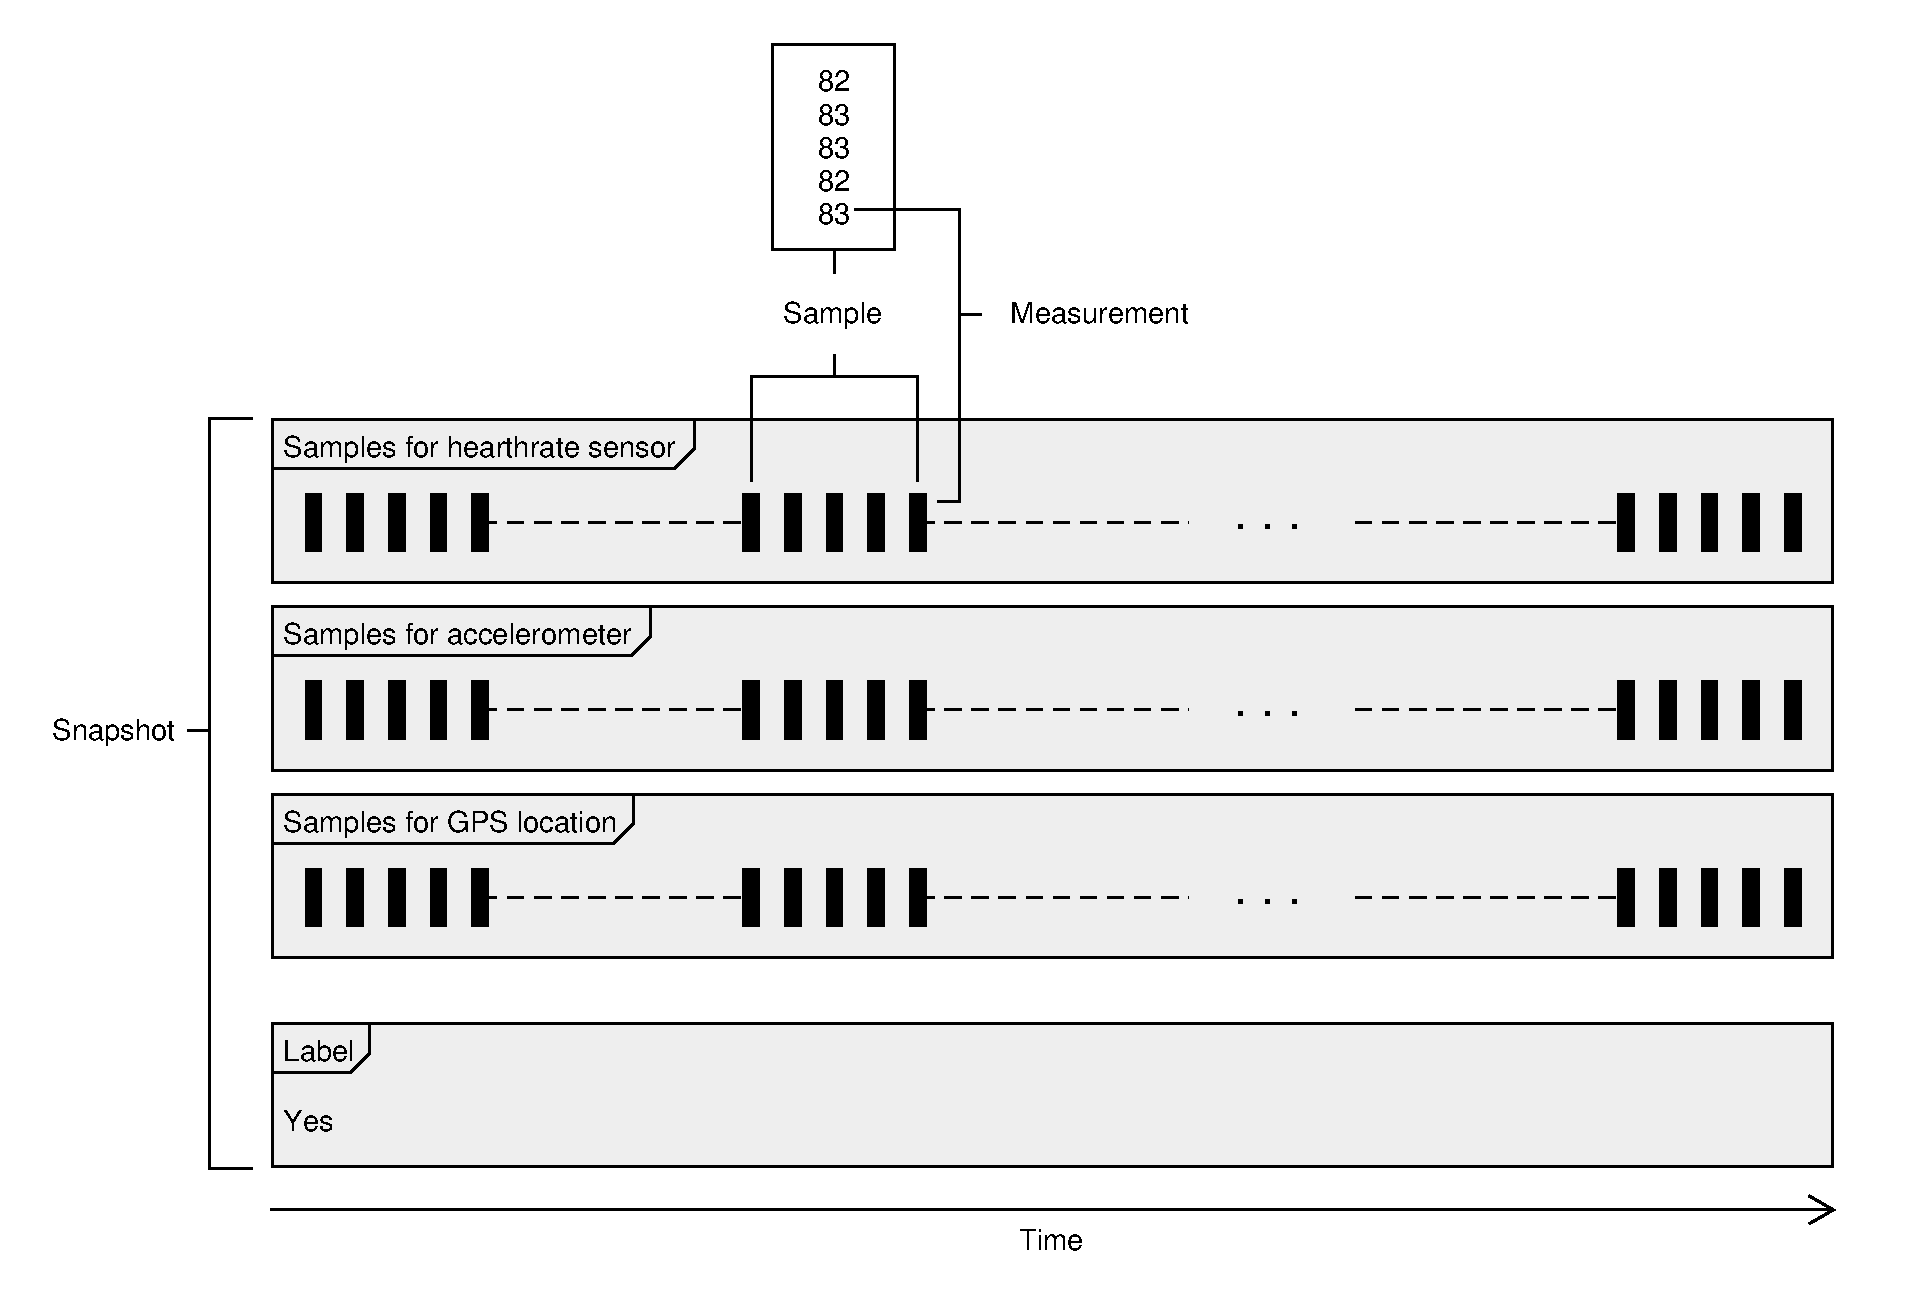
\includegraphics[width=\textwidth]{gathering_sensor_data/snapshot}
    \caption{Snapshot example containing measurements from three sensors and a label.}
    \label{fig:snapshot_example}
\end{figure}
\FloatBarrier

\todo[inline]{Beskriv hvad en campaign er i koden, brug gerne klassediagrammet til at forklare det!}

\begin{figure}[!htbp]
    \centering
    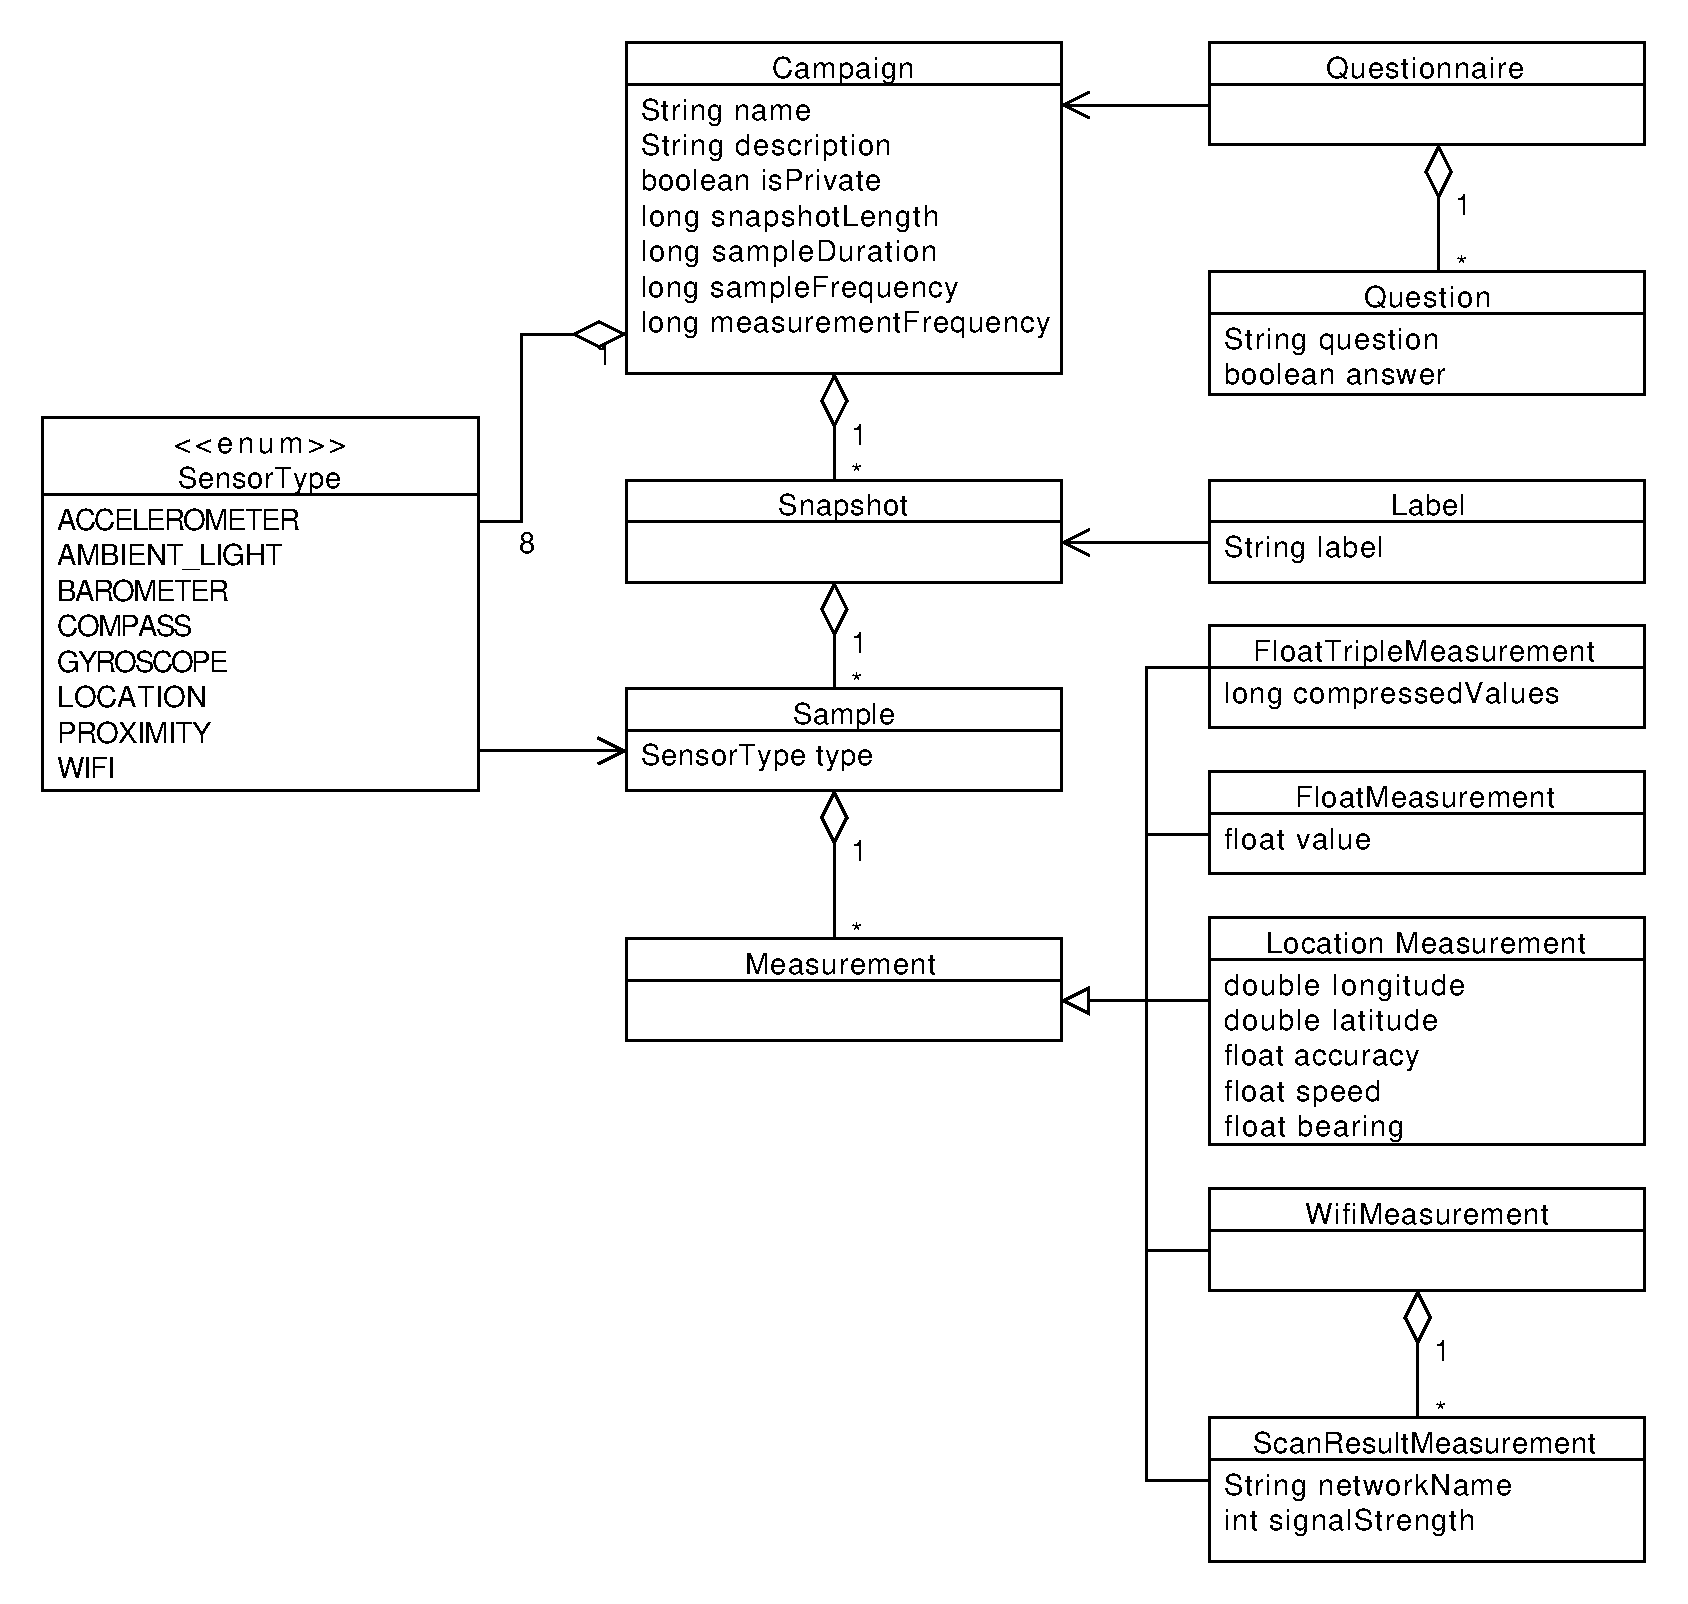
\includegraphics[width=\textwidth]{graphic/gathering_sensor_data/model_class_diagram.pdf}
    \caption{Class diagram of the campaign model.}
    \label{fig:model_class_diagram}
\end{figure}
\FloatBarrier

\todo[inline]{ref til figur}

\subsection{Questionnaires}
We had come to the conclusion that customers should be able to define questionnaires to be a part of the data collection \secref{sec:human_activity_recognition}. Customers should be able to define one or more separate questions or more generally data inputs which combined should make out a questionnaire model. 
\\\\
Simple boolean yes/no questions can directly be combined to create a discrete amount of labels or classes which can later be used as targets for an AI model but more open inputs, which for instance can be used for regression or as more diverse features, should also be possible. \todo{Overvej om vi når at implementere continuous inputs}
\\\\
A questionnaire specification should be transformable to a format which can be easily be parsed and send from the server to the collecting devices. We have therefore implemented a questionnaire to be Java Parcelable. \todo{Overvej at ændre det her hvis vi gør det til JSON ting i stedet}

